\documentclass[12pt]{report}
\usepackage{lingmacros}
\usepackage{tree-dvips}
\usepackage{graphicx}
\usepackage{listings}
\graphicspath{ {images/} }

\begin{document}

\section*{Report Labwork IX}

\subsection*{I: Which normal form does the employee database satisfy?, Why?}

\textbf{Employees database satisfy with level 3 of normal form. But it not fully.}

Explain:
{\small
\enumsentence{Each 4 unique entity: salaries, title, deparments and employees split to seprate table, each table have many property belong to that table}}

{\small
\enumsentence{Employees referent to tilte tables and salaries by emp\_no collumn, so we can fine what tilte of each employess, and one employees can have more than 1 title}}

{\small
\enumsentence{We have dept\_emp and dept\_manager to turn realation between employees and departments become 1-many and have date property for that. The same thing with dept\_manager}}



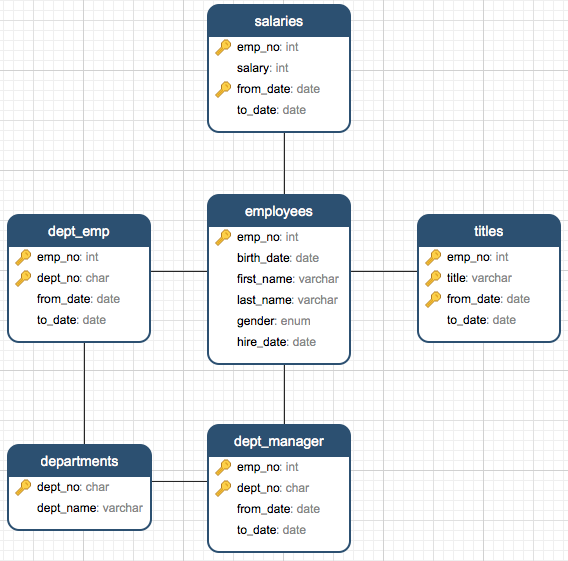
\includegraphics[width=0.8\paperwidth]{employees}


\subsection*{II: Produde a 3NF of the following Order form document by normalization}

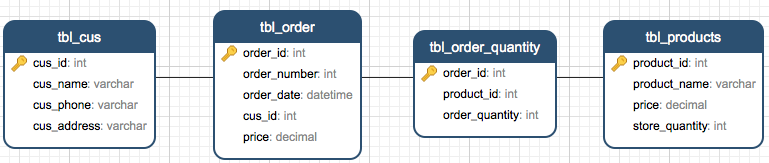
\includegraphics[width=0.8\paperwidth]{design}

Explain:
{\small
\enumsentence{We have many customers information but each customer can have many of order So we need to seprate customers information and assign cus\_id for each customer}}

{\small
\enumsentence{Each order can have many product with different quantity, but each order always have total price. Then we need price in tbl\_order, and separate the products quantity of each order to new table}}


{\small
\enumsentence{And the last tables tbl\_products will store all products detail information.}}

\end{document}